\documentclass[a4paper, 14pt]{extarticle}

\usepackage{../latexDependencies/misc/preamble}

\geometry{a4paper}

% Название дисциплины
\newcommand{\subject}{Теория вероятности и математическая статистика} 

% Тип работы
% lab - для лабораторной работы 
% hw  - для домашней     работы
\newcommand{\task}{lab} 

% Номер работы
\newcommand{\taskNumber}{1} 

% Название работы
\newcommand{\taskName}{Первоначальная обработка статистических данных} 

% Имя студента
\newcommand{\studentName}{Очкин Н.В.}

% Имя преподававателя
\newcommand{\teacherName}{Облакова Т.В.}

% Группа
\newcommand{\group}{ФН11-52Б}

% Вариант
\newcommand{\variant}{9}

\begin{document}

\graphicspath{ {../latexDependencies/images} } 
\normalsize

\newcommand{\printTask}{%
    \ifthenelse{\equal{\task}{lab}}{%
        лабораторной%
    }{%
        \ifthenelse{\equal{\task}{hw}}{%
            домашней%
        }{%
            Неизвестный тип задания%
        }%
    }%
}

\begin{titlepage}

    \begin{center}
        {\footnotesize \itshape Федеральное государственное бюджетное 
                       образовательное учреждение высшего образования}
    \end{center}

    \begin{minipage}[c]{0.1\textwidth}
        
\includegraphics[width=1.1\textwidth]{iconBMSTU}
    \end{minipage}
    \hfill
    \begin{minipage}[c]{0.9\textwidth}
        \centering
        \itshape
        \bfseries
        \small
        \guillemotleft Московский государственный технический университет \\
        имени Н.Э. Баумана\guillemotright \\
        (национальный исследовательский университет) \\
        (МГТУ им. Н.Э. Баумана) 
    \end{minipage}

    \vspace{0.5cm}
    \noindent\rule{\textwidth}{2pt} \\

    \noindent\uline{\textbf{ФАКУЛЬТЕТ} ФУНДАМЕНТАЛЬНЫЕ НАУКИ} \\
    \vspace{-5pt} \\
    \noindent\uline{\textbf{КАФЕДРА} ВЫЧИСЛИТЕЛЬНАЯ МАТЕМАТИКА И МАТЕМАТИЧЕСКАЯ} \\
    \vspace{-5pt} \\
    \noindent\uline{ФИЗИКА (ФН11)} \\
    \vspace{-5pt} \\
    \noindent\uline{\textbf{НАПРАВЛЕНИЕ ПОДГОТОВКИ} МАТЕМАТИКА И КОМПЬЮТЕРНЫЕ} \\
    \vspace{-5pt} \\
    \noindent\uline{НАУКИ (02.03.01)} \\

    \begin{center}
        \bfseries
        \textsc{О т ч е т} \\[10pt]
        по \printTask {} работе \textnumero {} \taskNumber
    \end{center}

    \vspace{10pt}

    \hspace{10pt} 
    \noindent \textbf{Название \printTask {} работы:} \par
    \vspace{5pt}
    \hspace{10pt} 
    \noindent \textbf{\uline{\taskName}}

    \vspace{10pt}

    \begin{center}
        \bfseries
        Вариант \textnumero {} \variant
    \end{center}

    \vspace{20pt}

    \hspace{10pt} 
    \noindent \textbf{Дисциплина:} \par
    \vspace{5pt}
    \hspace{10pt} 
    \noindent \subject

    \vspace{10pt}

    \begin{flushright}
        \renewcommand{\arraystretch}{3}
        \begin{tabular}{r r r}
            \multicolumn{1}{l}{Студент группы \uline{\group}} & 
            $\quad \underset{\text{(Подпись, дата)}}{\underline{\hspace{3cm}}} \quad$ & 
            \multicolumn{1}{c}{$\underset{\text{(И.О. Фамилия)}}{\uline{\textbf{\studentName}}}$} \\

            \multicolumn{1}{l}{Преподаватель} & 
            $\quad \underset{\text{(Подпись, дата)}}{\underline{\hspace{3cm}}} \quad$ & 
            \multicolumn{1}{c}{$\underset{\text{(И.О. Фамилия)}}{\uline{\textbf{\teacherName}}}$} \\
        \end{tabular}
    \end{flushright}

    \vfill

    \begin{center}
        \small
        Москва, 2024
    \end{center}
\end{titlepage}


% Reset the font size and page margins
\newgeometry{left=25mm, right=25mm, top=20mm, bottom=20mm}
% \fontsize{12pt}{16pt}\selectfont

\graphicspath{ {../latexDependencies/images/LW1} }

% Customize subsection style
\titleformat{\subsection}
  {\normalfont\normalsize\bfseries}{\thesubsection}{1em}{}

\thispagestyle{empty}

\null\newpage

\pagenumbering{roman}

\tableofcontents
\newpage

\pagenumbering{arabic}
\setcounter{page}{1}

\setstretch{1}
\linespread{1.1}

\setlength{\parindent}{0pt}

% --------------------------------------START--------------------------------------

\fontsize{12pt}{16pt}\selectfont

\section{Задание}

По данной выборке

\begin{enumerate}
    \item Найдите крайние члены вариационного ряда и размах выборки
    \item Осуществите группировку данных (количество интервалов 
    находим по правилу Стерджеса) 
    \item По сгруппированным данным постройте гистограмму 
    относительных частот
    \item Вычислите выборочное среднее и выборочную дисперсию.
    \item По виду гистограммы определите возможный закон распределения, 
    оцените параметры этого закона по методу моментов, постройте совмещенные 
    графики гистограммы и плотности предполагаемого закона
    \item Найдите эмпирическую функцию распределения и постройте совмещенные 
    графики эмпирической и теоретической функций распределения
\end{enumerate}

\section{Исходные данные}

\begin{center}
    \begin{table}[h!]
        \begin{adjustbox}{max width=\textwidth}
            \begin{tabular}{|c|c|c|c|c|c|c|c|c|c|c|}
                \hline
                14.495 & 4.715 & 7.175 & 8.428 & 11.093 &
                3.375 & 12.906 & 8.415 & 8.916 & 13.48 \\
                \hline
                5.343 & 17.985 & 15.992 & 13.89 & 9.838 &
                13.924 & 9.012 & 9.458 & 17.69 & 6.542 \\
                \hline
                14.396 & 8.592 & 8.206 & 14.237 & 7.357 &
                10.821 & 12.767 & 16.058 & 12.959 & 4.354 \\
                \hline
                12.888 & 10.268 & 9.182 & 5.647 & 8.282 &
                2.903 & 15.988 & 12.959 & 14.919 & 6.339 \\
                \hline
                2.375 & 17.921 & 9.097 & 15.85 & 11.449 &
                11.095 & 9.493 & 12.175 & 7.479 & 13.535 \\
                \hline
                9.234 & 6.078 & 4.964 & 6.355 & 13.957 &
                12.911 & 15.694 & 14.286 & 9.869 & 5.175 \\
                \hline
                5.811 & 7.241 & 5.814 & 3.086 & 6.875 &
                3.878 & 5.333 & 15.134 & 12.924 & 9.159 \\
                \hline
                4.727 & 4.646 & 15.535 & 9.919 & 17.117 &
                10.351 & 16.892 & 12.423 & 10.511 & 4.942 \\
                \hline
                4.843 & 9.927 & 15.864 & 3.635 & 17.963 &
                8.25 & 5.14 & 6.734 & 12.622 & 13.325 \\
                \hline
                3.377 & 16.195 & 12.04 & 12.768 & 2.744 &
                14.186 & 9.354 & 15.439 & 14.612 & 15.649 \\
                \hline
                8.681 & 5.006 & 3.608 & 2.867 & 12.177 &
                15.506 & 7.683 & 14.022 & 17.103 & 8.905 \\
                \hline
                12.173 & 17.757 & 6.883 & 2.666 & 9.861 &
                5.743 & 16.175 & 15.308 & 7.039 & 15.238 \\
                \hline
            \end{tabular}
        \end{adjustbox}
        \caption{Исходные данные}
        \label{tab:data}
    \end{table}
\end{center}

\newpage

\section{Решение}
Данная работа была выполнена с использованием языка программирования 
\textsc{python} и следующих модулей и библиотек: 

\renewcommand{\labelitemi}{\scalebox{0.5}{$\bullet$}}

\begin{center}
    \begin{multicols}{4}
        \begin{itemize}[itemsep=0pt]
            \item numpy
            \item pandas
            \item matplotlib
            \item scipy
            \item IPython
            \item math
            \item pyplot
            \item display
            \item stats
        \end{itemize}
    \end{multicols}
\end{center}

\subsection{Найдите крайние члены вариационного ряда и размах выборки}

Обратимся к листингу \ref{lst:3} и найдем крание члены вариационного ряда 
как минимальное и максимальное значения набора данных, а также размах выборки, 
как их разницу.
\begin{align*}
    & \text{Крайние члены: }  2.375, \hspace{5pt} 17.985 \\
    & \text{Размах выборки: }  15.61
\end{align*}

\subsection{Осуществите группировку данных}

Для начала определим количество интервалов, воспользовавшись правилом
Стерджеса:
\begin{equation*}
    n = 1 + \lfloor \log_2 N \rfloor,
\end{equation*}
где $N$ — общее число наблюдений величины, \\ 
$\log_2$ — логарифм по основанию 2, \\
$\lfloor x \rfloor$ — обозначает целую часть числа $x$. \\

И определим шаг интервала разделив размах выборки на количество интервалов.
Все операции представлены в листинге \ref{lst:4}.

\begin{align*}
    & \text{Количество интервалов: } 7 \\
    & \text{Шаг интервала: }  2.23
\end{align*}

Теперь сгруппируем данные. Алгоритм группировки, представленный в листингах 
\ref{lst:5} и \ref{lst:6}, опишем в виде псевдокода:

\begin{tcolorbox}[colback=gray!10, colframe=gray!50, title=Псевдокод алгоритма группировки данных]
    \begin{verbatim}
интервалы = [i для i в диапазоне от 1 до k включительно]

интервалы = []
частоты = []
относительныеЧастоты = []
серединыИнтервалов = []

текущий = минимальныйЭлемент
пока текущий + шаг <= максимальныйЭлемент:
    первыйЭлемент = текущий
    второйЭлемент = текущий + шаг

    интервалы.добавить(первыйЭлемент, второйЭлемент)

    серединаИнтервала = (первыйЭлемент + второйЭлемент) / 2
    серединыИнтервалов.добавить(серединаИнтервала)

    частота = найтиЧастоту(первыйЭлемент, второйЭлемент, данные)
    частоты.добавить(частота)

    относительнаяЧастота = частота / общееКоличествоЭлементов
    относительныеЧастоты.добавить(относительнаяЧастота)

    текущий = текущий + шаг

функция найтиЧастоту(минимальный, максимальный, данные):
    счетчик = 0

    для элемента в данные:
        если минимальный <= элемент < максимальный:
            счетчик += 1

    вернуть счетчик        
    \end{verbatim}
\end{tcolorbox}

\newpage

Представим полученную группировку в виде таблицы:

\begin{table}[h!]
    \centering
    \renewcommand{\arraystretch}{1.5}
    \begin{adjustbox}{max width=0.8\textwidth}
        \begin{tabular}{|c|c|c|c|c|c|}
        \hline
        номер & \multirow{2}{*}{интервал} & середина & \multirow{2}{*}{частота} & относительная \\
        интервала & & интервала & & частота \\
        \hline
        0 & [2.375; 4.605) & 3.490 & 12 & 0.100 \\
        \hline
        1 & [4.605; 6.835) & 5.720 & 20 & 0.167 \\
        \hline
        2 & [6.835; 9.065) & 7.950 & 18 & 0.150 \\
        \hline
        3 & [9.065; 11.295) & 10.180 & 18 & 0.150 \\
        \hline
        4 & [11.295; 13.525) & 12.410 & 17 & 0.142 \\
        \hline
        5 & [13.525; 15.755) & 14.640 & 20 & 0.167 \\
        \hline
        6 & [15.755; 17.985) & 16.870 & 14 & 0.117 \\
        \hline
        \end{tabular}
    \end{adjustbox}
    \caption{Сгруппированные данные}
    \label{tab:your_table_label}
\end{table}

А также найдем границы интервалов (листинг \ref{lst:8}):
\begin{equation*}
    [ 2.375 \hspace{10pt}  4.605 \hspace{10pt}  6.835 \hspace{10pt}  9.065 \hspace{10pt} 11.295 \hspace{10pt} 13.525 \hspace{10pt} 15.755 \hspace{10pt} 17.985]
\end{equation*}

\subsection{По сгруппированным данным постройте гистограмму относительных частот}

Воспользуемся библиотекой \textsc{matplotlib} для построения гистограммы (листинг \ref{lst:9})

\begin{center}
    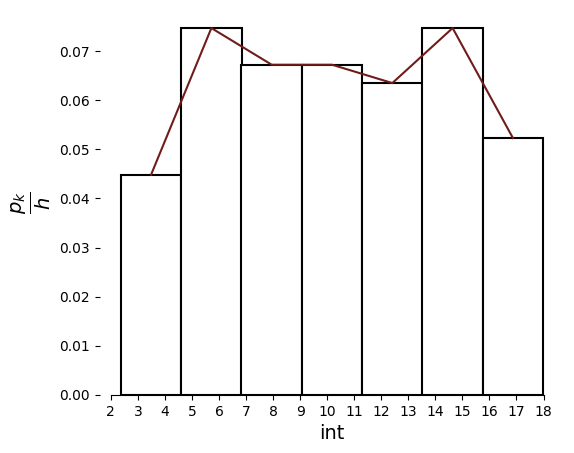
\includegraphics[width=0.8\textwidth]{LW1_15_1}
\end{center}

\subsection{Вычислите выборочное среднее и выборочную дисперсию}

По следющим формулам определим выборочное среднее и выборочную дисперсию 
соответственно:

\begin{equation*}
    \overline{X} = \frac{1}{n} \sum_{k=1}^{n} X_k \hspace{50pt}
    S^2 = \cfrac{1}{n - 1} \sum_{k=1}^{n} (X_k - \overline{X})^2
\end{equation*}

\vspace{15pt}

Обратимся к листингу \ref{lst:10} для вычислений:

\vspace{-15pt}

\begin{align*}
    & \text{Выборочное среднее: } 10.2681 \\
    & \text{Выборочная дисперсия: }  19.611
\end{align*}

\subsection{По виду гистограммы определите возможный закон распределения, 
оцените параметры этого закона по методу моментов, постройте совмещенные 
графики гистограммы и плотности предполагаемого закона}

Поскольку по виду гистограммы затруднительно дать точный ответ к какому
закону распределения относится заданная выборка данных, воспользуемся 
критерием Колмогорова-Смирнова. В качестве гипотез выберем следующие часто 
встречающиеся законы распределения:

\begin{center}
    \begin{multicols}{3}
        \begin{itemize}[itemsep=10pt]
            \item Нормальный
            \item Хи-квадрат
            \item Экспоненциальный
            \item Гамма
            \item Пуассоновский
            \item Равномерный
            \item t-распределение Стьюдента
            \item Логнормальный
            \item Бета
            \item Распределение Вейбулла
        \end{itemize}
    \end{multicols}
\end{center}

Применять критерий Колмогорова-Смирнова будем при помощи функции \textsc{kstest}
модуля \textsc{stats} библиотеки \textsc{scipy}, которая на выходе дает 4 
параметра:
\begin{enumerate}
    \item \textsc{statistic} \textbf{(или D)} - это основная статистика теста Колмогорова-Смирнова:
    \begin{itemize}
        \item Она представляет собой максимальную разницу между эмпирической 
        функцией распределения (наблюдаемые данные) и теоретической функцией 
        распределения.
        \item Значение лежит в диапазоне от 0 до 1. Чем больше значение, 
        тем сильнее различие между данными и теоретическим распределением.
    \end{itemize}

    \item \textsc{pvalue} - это значение p-уровня значимости:
    \begin{itemize}
        \item Оно показывает вероятность того, что наблюдаемое различие 
        между эмпирическим и теоретическим распределениями могло возникнуть 
        случайно при условии, что нулевая гипотеза (о соответствии распределению) 
        верна.
        \item Если \textsc{pvalue} меньше заранее установленного уровня 
        значимости (в нашем случае, 0.05), то нулевая гипотеза отвергается, 
        что означает, что данные не соответствуют предполагаемому распределению.
    \end{itemize}

    \item \textsc{statistic-location} - это точка, в которой наблюдается 
    максимальная разница между эмпирической и теоретической функциями 
    распределения:
    \begin{itemize}
        \item Это помогает понять, на каком участке распределения данные 
        сильнее всего отличаются от теоретической модели.
    \end{itemize}

    \item \textsc{statistic-sign} - это знак отклонения в точке максимальной 
    разницы:
    \begin{itemize}
        \item Может принимать значения 1 или -1.
        \item Если \textsc{statistic-sign} = -1, это означает, что в точке 
        максимального отклонения эмпирическая функция распределения 
        ниже, чем теоретическая.
        \item Если бы значение было 1, это указывало бы на то, 
        что эмпирическая функция распределения выше, чем теоретическая 
        в этой точке.
    \end{itemize}
\end{enumerate}

Первоначальный подбор параметров для каждого из закона осуществим при помощи 
следующей функции: \textsc{scipy.stats.<ЗАКОН>.fit}. Далее вручную методом 
подгонки, смотря на график, подберем параметр еще лучше.\\

Для каждого проверяемого закона также построим совмещенный график с 
гистограммой исходных данных.\\
Код предоставлен в листингах \ref{lst:11} и \ref{lst:12}

\vspace{-10pt}

\newgeometry{left=15mm, right=15mm, top=10mm, bottom=20mm}

\begin{center}
    \scalebox{0.85}{
    \begin{minipage}{\textwidth} 
        \begin{multicols}{2}
            \begin{gather*}
                \textbf{Нормальный} \\
                \begin{aligned}
                    & \text{Среднее, } \mu: & 10.2681 \\
                    & \text{Стандратное отклонение, } \sigma: & 4.4284
                \end{aligned}\\\\\\
                \text{Результаты теста} \\
                \text{Колмогорова-Смирнова:} \\
                \begin{aligned}
                    & \text{statistic: } \hspace{60pt} & 0.08872 \\
                    & \text{pvalue: } \hspace{60pt} & 0.28428 \\
                    & \text{statistic-location: } \hspace{60pt} & 12.767 \\
                    & \text{statistic-sign: } \hspace{60pt} & -1 \\
                \end{aligned} \\\\
                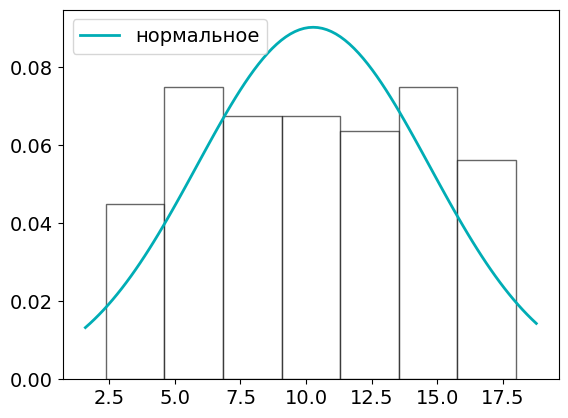
\includegraphics[width=0.4\textwidth]{LW1_22_5}
            \end{gather*}
            \vspace{-3pt}
            \begin{gather*}
                \textbf{Хи-квадрат} \\
                \begin{aligned}
                    & \text{Количество степеней свободы: } & 2 \\
                    & \text{Сдвиг : } & 2.375 \\
                    & \text{Параметр масштаба : } & 4.4099
                \end{aligned}\\\\
                \text{Результаты теста} \\
                \text{Колмогорова-Смирнова:} \\
                \begin{aligned}
                    & \text{statistic: } \hspace{60pt} & 0.17036 \\
                    & \text{pvalue: } \hspace{60pt} & 0.00163 \\
                    & \text{statistic-location: } \hspace{60pt} & 17.985 \\
                    & \text{statistic-sign: } \hspace{60pt} & 1 \\
                \end{aligned} \\\\
                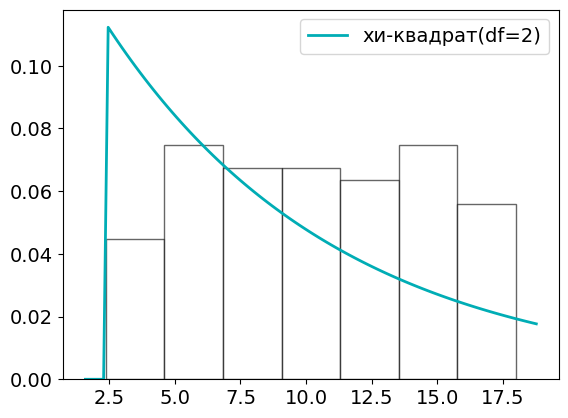
\includegraphics[width=0.4\textwidth]{LW1_22_11}
            \end{gather*}
        \end{multicols}
    \end{minipage}
    } 
\end{center}

\begin{center}
    \scalebox{0.85}{
    \begin{minipage}{\textwidth} 
        \begin{multicols}{2}
            \begin{gather*}
                \textbf{Экспоненциальный} \\
                \begin{aligned}
                    & \text{Сдвиг: } & 2.375 \\
                    & \text{Параметр масштаба, } \cfrac{1}{\lambda}: & 7.8931
                \end{aligned}\\\\
                \text{Результаты теста} \\
                \text{Колмогорова-Смирнова:} \\
                \begin{aligned}
                    & \text{statistic: } \hspace{60pt} & 0.18895 \\
                    & \text{pvalue: } \hspace{60pt} & 0.00032 \\
                    & \text{statistic-location: } \hspace{60pt} & 8.206 \\
                    & \text{statistic-sign: } \hspace{60pt} & -1 \\
                \end{aligned} \\\\
                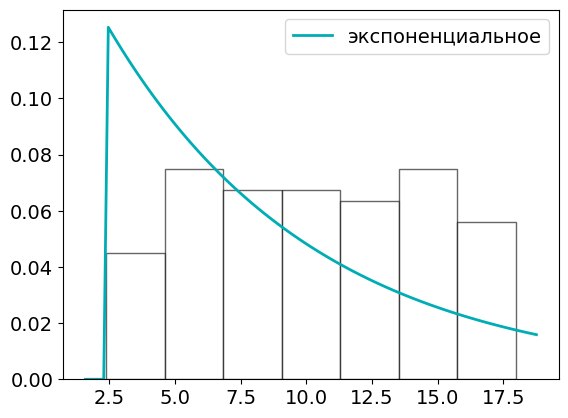
\includegraphics[width=0.4\textwidth]{LW1_22_17}
            \end{gather*}
            \vspace{-7pt}
            \begin{gather*}
                \textbf{Гамма} \\
                \begin{aligned}
                    & \text{Параметр формы: } & 2 \\
                    & \text{Сдвиг: } & 2.375 \\
                    & \text{Параметр масштаба: } & 4.4099
                \end{aligned}\\\\
                \text{Результаты теста} \\
                \text{Колмогорова-Смирнова:} \\
                \begin{aligned}
                    & \text{statistic: } \hspace{60pt} & 0.13175 \\
                    & \text{pvalue: } \hspace{60pt} & 0.02818 \\
                    & \text{statistic-location: } \hspace{60pt} & 17.985 \\
                    & \text{statistic-sign: } \hspace{60pt} & 1 \\
                \end{aligned} \\\\
                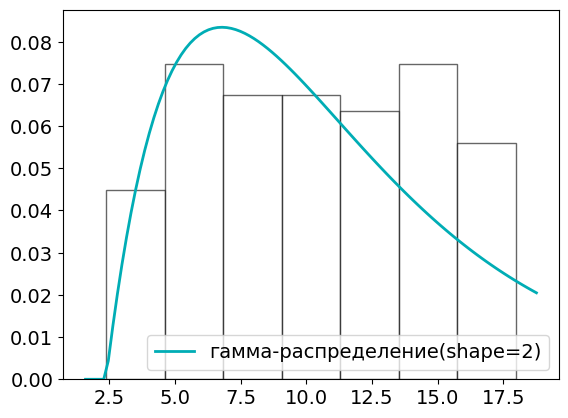
\includegraphics[width=0.4\textwidth]{LW1_22_23}
            \end{gather*}
        \end{multicols}
    \end{minipage}
    } 
\end{center}

\begin{center}
    \scalebox{0.85}{
    \begin{minipage}{\textwidth} 
        \begin{multicols}{2}
            \begin{gather*}
                \textbf{Пуассоновский} \\
                \begin{aligned}
                    & \text{Параметр интенсивности: } & 10.2681
                \end{aligned}\\\\\\
                \text{Результаты теста} \\
                \text{Колмогорова-Смирнова:} \\
                \begin{aligned}
                    & \text{statistic: } \hspace{60pt} & 0.19049 \\
                    & \text{pvalue: } \hspace{60pt} & 0.00027 \\
                    & \text{statistic-location: } \hspace{60pt} & 12.04 \\
                    & \text{statistic-sign: } \hspace{60pt} & -1 \\
                \end{aligned} \\\\
                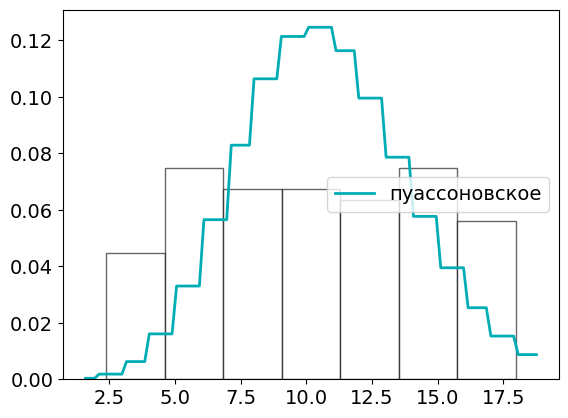
\includegraphics[width=0.4\textwidth]{LW1_22_29}
            \end{gather*}
            \vspace{0pt}
            \begin{gather*}
                \textbf{Равномерный} \\
                \begin{aligned}
                    & \text{Нижняя граница: } & 2.375 \\
                    & \text{Размах: } & 15.61 
                \end{aligned}\\\\
                \text{Результаты теста} \\
                \text{Колмогорова-Смирнова:} \\
                \begin{aligned}
                    & \text{statistic: } \hspace{60pt} & 0.048 \\
                    & \text{pvalue: } \hspace{60pt} & 0.93243 \\
                    & \text{statistic-location: } \hspace{60pt} & 16.195 \\
                    & \text{statistic-sign: } \hspace{60pt} & 1 \\
                \end{aligned} \\\\
                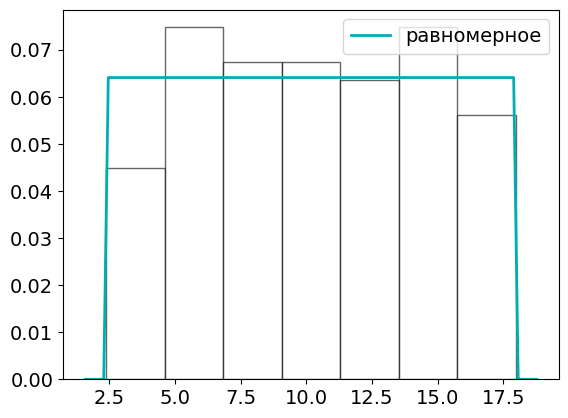
\includegraphics[width=0.4\textwidth]{LW1_22_35}
            \end{gather*}
        \end{multicols}
    \end{minipage}
    } 
\end{center}

\begin{center}
    \scalebox{0.85}{
    \begin{minipage}{\textwidth} 
        \begin{multicols}{2}
            \begin{gather*}
                \textbf{t-распределение Стьюдента} \\
                \begin{aligned}
                    & \text{Кол-во степеней свободы: } & 2 \\
                    & \text{Сдвиг: } & 10.2681 \\
                    & \text{Масштаб: } & 4.4099 
                \end{aligned}\\\\
                \text{Результаты теста} \\
                \text{Колмогорова-Смирнова:} \\
                \begin{aligned}
                    & \text{statistic: } \hspace{60pt} & 0.11112 \\
                    & \text{pvalue: } \hspace{60pt} & 0.09562 \\
                    & \text{statistic-location: } \hspace{60pt} & 17.985 \\
                    & \text{statistic-sign: } \hspace{60pt} & 1 \\
                \end{aligned} \\\\
                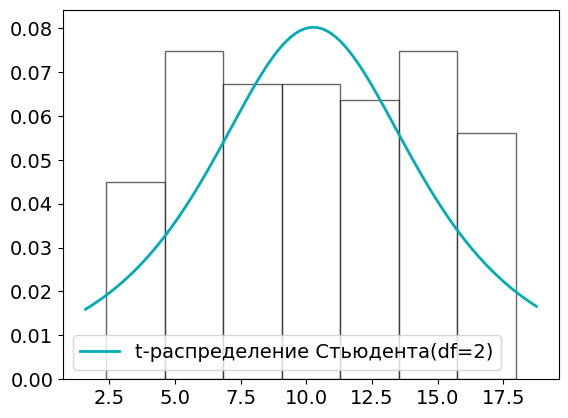
\includegraphics[width=0.4\textwidth]{LW1_22_41}
            \end{gather*}
            \vspace{0pt}
            \begin{gather*}
                \textbf{Логнормальный} \\
                \begin{aligned}
                    & \text{Параметр формы: } & 0.515 \\
                    & \text{Сдвиг: } & 2.375 \\
                    & \text{Параметр масштаба: } & 9.1469
                \end{aligned}\\\\
                \text{Результаты теста} \\
                \text{Колмогорова-Смирнова:} \\
                \begin{aligned}
                    & \text{statistic: } \hspace{60pt} & 0.19857 \\
                    & \text{pvalue: } \hspace{60pt} & 0.00013 \\
                    & \text{statistic-location: } \hspace{60pt} & 6.883 \\
                    & \text{statistic-sign: } \hspace{60pt} & 1 \\
                \end{aligned} \\\\
                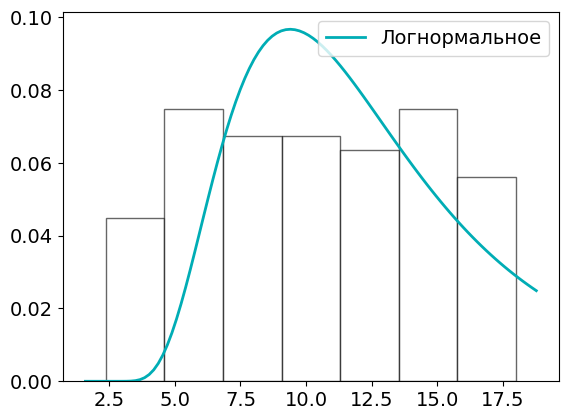
\includegraphics[width=0.4\textwidth]{LW1_22_47}
            \end{gather*}
        \end{multicols}
    \end{minipage}
    } 
\end{center}

\begin{center}
    \scalebox{0.85}{
    \begin{minipage}{\textwidth} 
        \begin{multicols}{2}
            \begin{gather*}
                \textbf{Бета} \\
                \begin{aligned}
                    & \text{Параметр формы 1: } & 1.2407 \\
                    & \text{Параметр формы 2: } & 0.9441 \\
                    & \text{Сдвиг: } & 0.924 \\
                    & \text{Масштаб: } & 17.0606
                \end{aligned}\\\\
                \text{Результаты теста} \\
                \text{Колмогорова-Смирнова:} \\
                \begin{aligned}
                    & \text{statistic: } \hspace{60pt} & 0.0842 \\
                    & \text{pvalue: } \hspace{60pt} & 0.34331 \\
                    & \text{statistic-location: } \hspace{60pt} & 9.927 \\
                    & \text{statistic-sign: } \hspace{60pt} & 1 \\
                \end{aligned} \\\\
                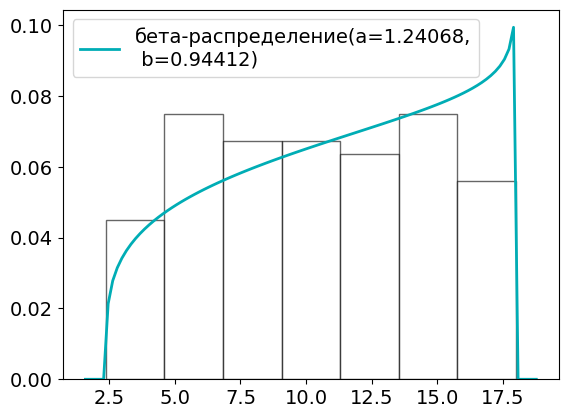
\includegraphics[width=0.4\textwidth]{LW1_22_53}
            \end{gather*}
            \vspace{0pt}
            \begin{gather*}
                \textbf{Вейбулловский} \\
                \begin{aligned}
                    & \text{Параметр формы: } & 2.4993 \\
                    & \text{Сдвиг: } & 2.375 \\
                    & \text{Параметр масштаба: } & 4.4099
                \end{aligned}\\\\\\
                \text{Результаты теста} \\
                \text{Колмогорова-Смирнова:} \\
                \begin{aligned}
                    & \text{statistic: } \hspace{60pt} & 0.5389 \\
                    & \text{pvalue: } \hspace{60pt} & 0.0 \\
                    & \text{statistic-location: } \hspace{60pt} & 8.905 \\
                    & \text{statistic-sign: } \hspace{60pt} & -1 \\
                \end{aligned} \\\\
                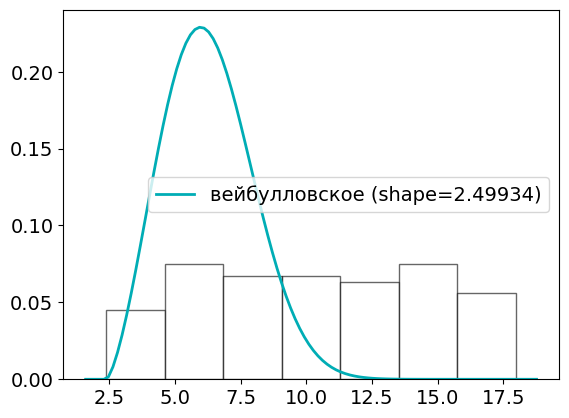
\includegraphics[width=0.4\textwidth]{LW1_22_59}
            \end{gather*}
        \end{multicols}
    \end{minipage}
    } 
\end{center}

\vspace{35pt}

Запишем все данные в таблицу

\vfill

\begin{table}[h!]
    \centering
    \renewcommand{\arraystretch}{1.5}
    \begin{adjustbox}{max width=0.8\textwidth}
        \begin{tabular}{|c|c|c|c|c|c|}
        \hline
        \textbf{Index} & \textbf{Name} & \textbf{Statistic} & \textbf{P-Value} & \textbf{Statistic Location} & \textbf{Statistic Sign} \\
        \hline
        0 & norm & 0.089 & 0.284 & 12.767 & -1 \\
        \hline
        1 & chi2 & 0.170 & 0.002 & 17.985 & 1 \\
        \hline
        2 & expon & 0.189 & 0.000 & 8.206 & -1 \\
        \hline
        3 & gamma & 0.132 & 0.028 & 17.985 & 1 \\
        \hline
        4 & poisson & 0.190 & 0.000 & 12.040 & -1 \\
        \hline
        5 & uniform & 0.048 & 0.932 & 16.195 & 1 \\
        \hline
        6 & t & 0.111 & 0.096 & 17.985 & 1 \\
        \hline
        7 & lognorm & 0.199 & 0.000 & 6.883 & 1 \\
        \hline
        8 & beta & 0.084 & 0.343 & 9.927 & 1 \\
        \hline
        9 & weibull\_min & 0.539 & 0.000 & 8.905 & -1 \\
        \hline
        \end{tabular}
    \end{adjustbox}
    \caption{Результаты критерия Колмогорова-Смирнова}
    \label{tab:statistical_data1}
\end{table}

\vspace{20pt}

\newgeometry{left=25mm, right=25mm, top=20mm, bottom=20mm}

Избавимся от строк таблицы со значениями \textsc{p-value} < 0.05

\begin{table}[h!]
    \centering
    \renewcommand{\arraystretch}{1.5}
    \begin{adjustbox}{max width=0.8\textwidth}
        \begin{tabular}{|c|c|c|c|c|c|}
        \hline
        \textbf{Index} & \textbf{Name} & \textbf{Statistic} & \textbf{P-Value} & \textbf{Statistic Location} & \textbf{Statistic Sign} \\
        \hline
        0 & norm & 0.089 & 0.284 & 12.767 & -1 \\
        \hline
        5 & uniform & 0.048 & 0.932 & 16.195 & 1 \\
        \hline
        6 & t & 0.111 & 0.096 & 17.985 & 1 \\
        \hline
        8 & beta & 0.084 & 0.343 & 9.927 & 1 \\
        \hline
        \end{tabular}
    \end{adjustbox}
    \caption{Отфильтрованные результаты критерия Колмогорова-Смирнова}
    \label{tab:statistical_data2}
\end{table}

\vspace{20pt}

Отсортируем по значению \textsc{statistic} в порядке убывания

\begin{table}[h!]
    \centering
    \renewcommand{\arraystretch}{1.5}
    \begin{adjustbox}{max width=0.8\textwidth}
        \begin{tabular}{|c|c|c|c|c|c|}
        \hline
        \textbf{Index} & \textbf{Name} & \textbf{Statistic} & \textbf{P-Value} & \textbf{Statistic Location} & \textbf{Statistic Sign} \\
        \hline
        5 & uniform & 0.048 & 0.932 & 16.195 & 1 \\
        \hline
        8 & beta & 0.084 & 0.343 & 9.927 & 1 \\
        \hline
        0 & norm & 0.089 & 0.284 & 12.767 & -1 \\
        \hline
        6 & t & 0.111 & 0.096 & 17.985 & 1 \\
        \hline
        \end{tabular}
    \end{adjustbox}
    \caption{Отсортированные результаты критерия Колмогорова-Смирнова}
    \label{tab:statistical_data3}
\end{table}

\vspace{20pt}

Исходя из полученных данных, можно сделать вывод, что закон распределения выборки
с наибольшей вероятностью является \textbf{равномерным}, далее \textbf{бета-распределением},
\textbf{нормальным} и, наконец, \textbf{t-распределением Стьюдента} (с указанными ранее
параметрами).\\

Изобразим плотности первых трех законов на совмещенном графике с гистограммой, построенной
на заданной выборке данных (листинг \ref{lst:13})

\begin{center}
    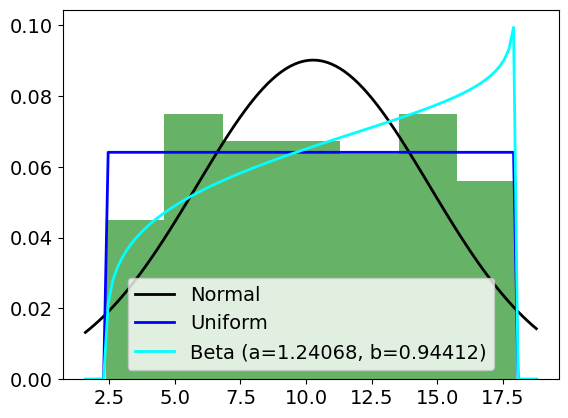
\includegraphics[width=0.7\textwidth]{LW1_25_0.png}
\end{center}

Оценим параметры равномерного закона распределения методом моментов

\begin{gather*}
    M_{\xi} = \int_{-\inf}^{+\inf} x p_{\xi} (x) dx = 
    \int_{a}^{b} x \cdot \cfrac{1}{b-a} dx = \cfrac{a + b}{2} \\\\
    M_{\xi} = \overline{X} \Longrightarrow \cfrac{a + b}{2} = \overline{X} 
    \Longrightarrow a + b = 2 \overline{X} \approx 20.5362 \\\\
    D_{\xi} = M_{\xi}^2 - (M_{\xi})^2 \\\\
    M_{\xi}^2 = \int_{-\inf}^{+\inf} x^2 p_{\xi} (x) dx = 
    \int_{a}^{b} x^2 \cdot \cfrac{1}{b-a} dx = \cfrac{a^2 + ab + b^2}{3} \\\\
    (M_{\xi})^2 = \cfrac{(a + b)^2}{4} \\\\
    D_{\xi} = \cfrac{(b - a)^2}{12} \\\\
    D_{\xi} = S^2 \Longrightarrow \cfrac{(b - a)^2}{12} = S^2 
    \Longrightarrow (b - a)^2 = 12 S^2 \Longrightarrow b - a = 2 \sqrt{3} \sqrt{S^2}
    \approx 15.3405
\end{gather*}

\begin{equation*}
    \begin{cases}
        b - a = 15.3405 \\
        b + a = 20.5362
    \end{cases} 
\end{equation*}

\begin{equation*}
    \begin{cases}
        a = 2.59785 \\
        b = 17.93835
    \end{cases} 
\end{equation*}\\

(Можно заметить, что найденные параметры не сильно отличаются от тех, что были
найдены программно)

\subsection{Найдите эмпирическую функцию распределения и постройте 
совмещенные графики эмпирической и теоретической функций распределения}

Запишем реализацию эмпирической функции распределения femp(x) в виде 
псевдокода:

\begin{tcolorbox}[colback=gray!10, colframe=gray!50, title=Псевдокод функции femp]
    \begin{verbatim}
функция femp(x) {
    функция ind(x) {
        возвращает 1 если x > 0, иначе возвращает 0
    }

    сумма = 0
    для i в диапазоне (количества интервалов) {
        сумма += i-й элемент вектора относительных частот * \ 
                    ind(x минус i-й элемент вектора с \
                                серединами интервалов)
    }

    вернуть сумму
}      
    \end{verbatim}
\end{tcolorbox}

Сам же код реализации функции предоставлен в листинге \ref{lst:14}.\\

Построим совмещенные графики эмпирической функции распределения и 
функции распределения для равномерного закона (a = 2.59785, b = 17.93835), 
воспользовавшись 
листингами \ref{lst:15} и \ref{lst:16}.

\begin{center}
    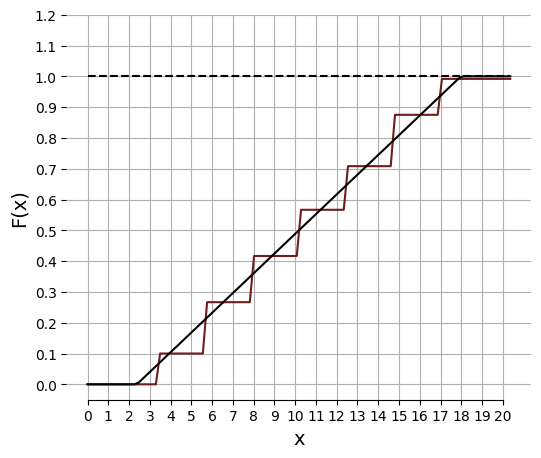
\includegraphics[width=0.7\textwidth]{LW1_31_0}
\end{center}

Теперь тоже самое, но для нормального закона ($\mu$ = 10.2681, $\sigma^2$ = 19.6109) 
(листинги \ref{lst:15} и \ref{lst:17}).\\
{ \footnotesize \textbf{Примечание}: параметры были найдены с помощью библиотеки 
\textsc{scipy}}.

\begin{center}
    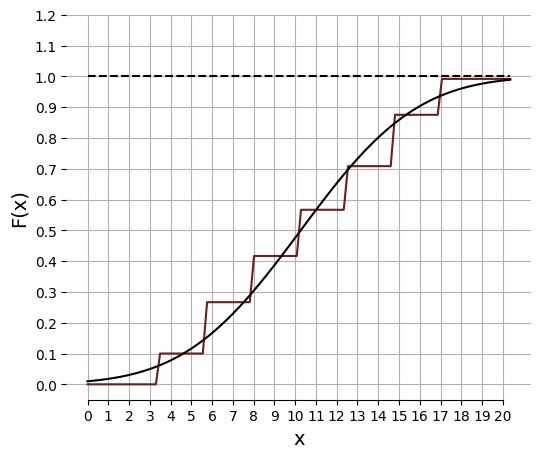
\includegraphics[width=0.7\textwidth]{LW1_32_0}
\end{center}

И для бета-распределения ($\alpha$ = 1.2407, $\beta$ = 0.94412, сдвиг (loc) = 2.375,
масштаб (scale) = 4.4099) 
(листинги \ref{lst:15} и \ref{lst:18}).\\
{ \footnotesize \textbf{Примечание}: параметры были найдены с помощью библиотеки 
\textsc{scipy}}.

\begin{center}
    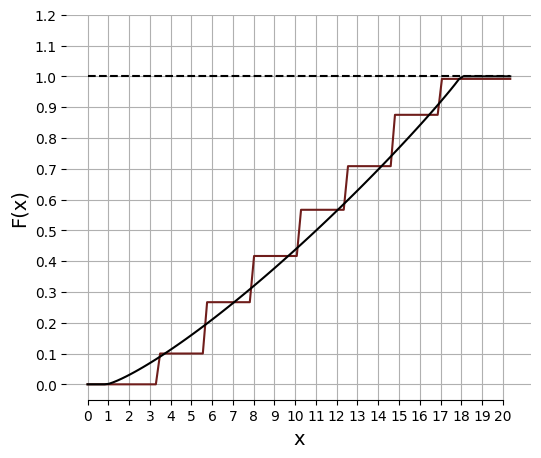
\includegraphics[width=0.7\textwidth]{LW1_33_0}
\end{center}

\subsection{Вывод}

Первоначальная обработка позволяет предварительно отнести выборку
(с наибольшей вероятностью) к равномерному закону с параметрами:
\begin{equation*}
    a = 2.59785 \qquad b = 17.93835
\end{equation*}

% --------------------------------------CODE---------------------------------------

\section{Приложение}

Программный код, с помощью которого была выполнена данная лабораторная работа.\\

\vspace{20pt}

\noindent \textbf{Примечание}.\\

\noindent Так как отчет был написан с использованием дистрибутива TeX и 
следующий код был отформатирован с использованием окружения \textsc{lstlisting}, 
в некоторых местах текст, написанный на русском языке, может иметь проблемы 
с выравниванием, пробелами, шрифтом и т.д. Это связано с тем, что библиотека 
\textsc{listings}, из которой мы берем окружение для форматирования кода, 
плохо работает с Unicode.

\vspace{20pt}

% \newgeometry{left=15mm, right=15mm, top=20mm, bottom=20mm}

\setstretch{1}

\lstdefinestyle{mystyle}{
    basicstyle=\ttfamily\footnotesize,
    keywordstyle=\color{blue},
    stringstyle=\color{red},
    commentstyle=\color{green!50!black},
    showstringspaces=false
}

% Set the style for Python code
\lstset{style=mystyle, language=Python, extendedchars=\true}

\begin{lstlisting}[caption={Подключение библиотек}, label={lst:1}]
import numpy as np
import pandas as pd
import matplotlib.pyplot as plt
import scipy as sp
import math
from IPython.display import display, Math

PRECISION = 5
pd.set_option('display.float_format', '{:.3f}'.format)
np.set_printoptions(precision=PRECISION)
\end{lstlisting}

\begin{lstlisting}[caption={Ввод данных}, label={lst:2}]
_data = [
    14.495, 4.715,  7.175,  8.428,  11.093, 3.375
    12.906, 8.415,  8.916,  13.48,  5.343,  17.985
    15.992, 13.89,  9.838,  13.924, 9.012,  9.458
    17.69,  6.542,  14.396, 8.592,  8.206,  14.237
    7.357,  10.821, 12.767, 16.058, 12.959, 4.354
    12.888, 10.268, 9.182,  5.647,  8.282,  2.903
    15.988, 12.959, 14.919, 6.339,  2.375,  17.921
    9.097,  15.85,  11.449, 11.095, 9.493,  12.175
    7.479,  13.535, 9.234,  6.078,  4.964,  6.355
    13.957, 12.911, 15.694, 14.286, 9.869,  5.175
    5.811,  7.241,  5.814,  3.086,  6.875,  3.878
    5.333,  15.134, 12.924, 9.159,  4.727,  4.646
    15.535, 9.919,  17.117, 10.351, 16.892, 12.423
    10.511, 4.942,  4.843,  9.927,  15.864, 3.635
    17.963, 8.25,   5.14,   6.734,  12.622, 13.325
    3.377,  16.195, 12.04,  12.768, 2.744,  14.186
    9.354,  15.439, 14.612, 15.649, 8.681,  5.006
    3.608,  2.867,  12.177, 15.506, 7.683,  14.022
    17.103, 8.905,  12.173, 17.757, 6.883,  2.666
    9.861,  5.743,  16.175, 15.308, 7.039,  15.238
]
\end{lstlisting}

\begin{lstlisting}
\begin{lstlisting}
# Variation series
_parsedData = [_data[i:i+10] for i in range(0, len(_data), 10)] 

_parsedData
\end{lstlisting}

\begin{center}
    1. Крайние члены вариационного ряда и размах выборки
\end{center}

\begin{lstlisting} [caption={Поиск крайних членов и размаха выборки}, label={lst:3}]
# Extreme members
_maxEl = np.max(_parsedData)
_minEl = np.min(_parsedData)

print(f"Крайние члены: {_maxEl}, {_minEl}")

# Sample range
_range = np.round(_maxEl - _minEl, PRECISION)

print(f"Размах выборки: {_range}")
\end{lstlisting}

\begin{center}
    2. Осуществите группировку данных
\end{center}

\begin{lstlisting}[caption={Поиск интервалов}, label={lst:4}]
# Let's find the number of intervals using Sturges' rule
_n = len(_data)
_k = 1 + np.trunc(np.log2(_n))

print(f"Количество интервалов: {_k}")

# Interval step
_h = _range / _k

print(f"Шаг интервала: {_h}")
\end{lstlisting}

\begin{lstlisting}[caption={Функция для нахождения частот}, label={lst:5}]
# function for finding frequencies
def findFrequency(minim, maxim, data):
    count = 0

    for el in data:
        if minim <= el < maxim:
            count += 1

    return count
\end{lstlisting}
    
\begin{lstlisting}[caption={Группировка данных}, label={lst:6}]
intervals           = [i for i in range(1, int(_k) + 1)] # interval number
tableRanges         = [] # interval
frequencies         = [] # frequency
relativeFrequencies = [] # relative frequency
midRanges           = [] # middle of the interval

curr = _minEl
while (math.floor(curr + _h) <= _maxEl):
    firstEl  = curr                        # first element of the current interval 
    secondEl = round(curr + _h, PRECISION) # second element of the current interval
    tableRanges.append((firstEl, secondEl))

    midRange = round((firstEl + secondEl)/2, PRECISION) # middle of the interval
    midRanges.append(midRange)

    frequency = findFrequency(firstEl, secondEl, _data) # frequency
    frequencies.append(frequency)                          
    
    relativeFrequency = round(frequency / _n, PRECISION) # relative frequency
    relativeFrequencies.append(relativeFrequency)

    curr = round(curr + _h, PRECISION)
\end{lstlisting}

\begin{lstlisting}[caption={Оформление данных в виде таблицы}, label={lst:7}]
_intervalRange = pd.DataFrame({'номер интервала':       intervals, 
                               'интервал':             tableRanges, 
                               'середина интервала':     midRanges,
                               'частота':              frequencies,
                               'относительная частота': relativeFrequencies})

_intervalRange
\end{lstlisting}

\begin{lstlisting}[caption={Поиск границ интервалов}, label={lst:8}]
# interval boundaries
_int1 = midRanges - _h/2
_int1 = np.append(_int1, _maxEl)

print(f'границы интервалов: {_int1}')
\end{lstlisting}

\begin{center}
    3. По сгруппированным данным постройте гистограмму относительных частот
\end{center}

\begin{lstlisting}
def buildLine(x, y, color):
    plt.plot(x, y, color=color, linestyle='-', linewidth=1.5)
\end{lstlisting}

\begin{lstlisting}[caption={Построение гистограммы}, label={lst:9}]
def buildBar(x, y, overlay = None, showAxis = True):
    RED   = '#6F1D1B'
    BLUE  = '#00ADB5'
    WHITE = '#EEEEEE'
    BLACK = '#393E46' # #253031 #0D1B1E #1C2321

    # Define font sizes
    SIZE_DEFAULT = 14
    SIZE_LARGE   = 16
    SIZE_TICKS   = 10
    plt.rc("font", weight="normal")        # controls default font
    plt.rc("font", size=SIZE_DEFAULT)      # controls default text sizes
    plt.rc("axes", titlesize=SIZE_LARGE)   # fontsize of the axes title
    plt.rc("axes", labelsize=SIZE_DEFAULT) # fontsize of the x and y labels
    plt.rc("xtick", labelsize=SIZE_DEFAULT)# fontsize of the tick labels
    plt.rc("ytick", labelsize=SIZE_DEFAULT)# fontsize of the tick labels

    fig, ax = plt.subplots(
        figsize=(6, 5)
    )

    xticks = [i for i in range(math.floor(min(x)) - 1, math.ceil(max(x)) + 2)]

    # Hide the all but the bottom spines (axis lines)
    ax.spines["right"].set_visible(False)
    ax.spines["left"].set_visible(False)
    ax.spines["top"].set_visible(False)

    if not showAxis:
        ax.spines["bottom"].set_visible(False)

    # Only show ticks on the left and bottom spines
    ax.yaxis.set_ticks_position("left")
    ax.xaxis.set_ticks_position("bottom")
    ax.spines["bottom"].set_bounds(min(xticks), max(xticks))

    # histogtamm 
    plt.bar(x, y, width=2.25, color='white', edgecolor='black', 
            linewidth=1.5, align='center')

    # line
    if overlay is None:
        buildLine(x, y, RED)
    else:
        xmin, xmax = plt.xlim()
        x = np.linspace(xmin, xmax, 100)
        calculate_y = overlay(x)
        plt.plot(x, calculate_y, color=BLUE, linestyle='-', linewidth=1.5)

    # axis names
    if showAxis:
        plt.xlabel('int')
        plt.ylabel('$\\frac{p_k}{h}$', fontsize=20)
        plt.xticks(xticks)
    else:
        ax.xaxis.set_ticks_position('none')
        ax.yaxis.set_ticks_position('none')
        ax.set_xticks([])
        ax.set_yticks([])

    # Adjust the font size of the tick labels
    plt.tick_params(axis='both', which='major', labelsize=SIZE_TICKS)

    plt.show()
\end{lstlisting}

\begin{lstlisting}
def overlayPlot(overlay):
    BLUE  = '#00ADB5'

    plt.hist(_data, bins=int(_k), color='white', edgecolor='black', 
             density=True, alpha=0.6)

    xmin, xmax = plt.xlim()
    x = np.linspace(xmin, xmax, 100)
    
    calculate_y, label = overlay(x)
    plt.plot(x, calculate_y, color=BLUE, linestyle='-', linewidth=2, label=label)

    plt.legend()
    plt.show()
\end{lstlisting}

\begin{lstlisting}
# is indicated along the ordinate axis when constructing a histogram
_histogrammOrdinateAxis = relativeFrequencies / _h

print(f'x: {midRanges}')
print(f'y: {_histogrammOrdinateAxis}')

buildBar(midRanges, _histogrammOrdinateAxis)
\end{lstlisting}

\begin{lstlisting}
plt.hist(_data, bins=int(_k))
plt.show()
\end{lstlisting}

\begin{center}
    4. Вычислите выборочное среднее и выборочную дисперсию
\end{center}

\begin{lstlisting}[caption={поиск выборочного среднего и выборочной дисперсии}, label={lst:10}]
# sample average
_overlineX = (1 / _n) * np.sum(_data) 

# sample variance
_S2 = 1 / (_n - 1) * np.sum((_data - _overlineX)**2)

print(f'выборочное среднее: {_overlineX}')
print(f'выборочная дисперсия: {_S2}')
\end{lstlisting}

\begin{center}
    5. По виду гистограммы определите возможный закон распределения, 
    оцените параметры этого закона по методу моментов, постройте совмещенные 
    графики гистограммы и плотности предполагаемого закона
\end{center}

\begin{lstlisting}[caption={Анализ и вывод полученных данных в ходе теста Колмогорова-Смирнова}, label={lst:11}]
def align(name, enName, kstestRes, *params):
    def line(n):
        display('-'*n)

    heading: str = f"\\begin{{equation}} " \
                   f"   \\text{{{name}}} " \
                   f"\\end{{equation}}   " \
    
    dataDisplay: str = f"\\begin{{align}}\n" 

    NAME   = 0
    SYMBOL = 1
    VALUE  = 2
    for param in params:
        dataDisplay += f"& \\text{{{param[NAME]}}}, "\
                       f"{param[SYMBOL]}: & \\quad {param[VALUE]} \\\\\n"

    dataDisplay += f"\\end{{align}}" 

    kstestHeading = \
    f"\\begin{{equation}} "                           \
    f"   \\text{{результаты теста Колмогорова-Смирнова}}: " \
    f"\\end{{equation}} "                                  

    statistic          = kstestRes.statistic
    pvalue             = kstestRes.pvalue
    statistic_location = kstestRes.statistic_location
    statistic_sign     = kstestRes.statistic_sign

    statisticDisplay = f'максимальное различие между эмпирической и '      \
                       f'теоретической функциями распределения составляет ' \
                       f'примерно: {int(np.round(statistic, 2) * 100)}\\%'

    pvalueFlag = True if pvalue < 0.05 else False

    pvalueDisplay = f'значение p-уровня значимости: {pvalue} '
    pvalueDisplay += '<' if pvalueFlag else '>'
    pvalueDisplay += f' 0.05'

    if pvalueFlag:
        pvalueDisplay += \
        f' (данные не соответствуют предполагаемому распределению.)'
    else:
        pvalueDisplay += \
        f' (на уровне значимости 0.05 нет оснований отвергнуть гипотезу ' \
        f'о соответствии данных выбранному распределению)'

    statistic_locationDisplay = \
    f'максимальное отклонение наблюдается при значении данных, ' \
    f'равном {statistic_location}'

    statistic_signDisplay = \
    f'в точке максимального отклонения эмпирическая функция распределения '
    statistic_signDisplay += 'ниже' if statistic_sign < 0 else 'выше'
    statistic_signDisplay += ', чем теоретическая'

    kstestResDisplay = [statisticDisplay, 
                        pvalueDisplay, 
                        statistic_locationDisplay, 
                        statistic_signDisplay]

    kstestDisplay  = f"\\begin{{align}}\n" 

    for res in kstestResDisplay:
        kstestDisplay += f"& \\text{{{res}}} \\\\\n"

    kstestDisplay += f"\\end{{align}}" 

    line(200)

    display(Math(heading))
    display(Math(dataDisplay))
    display(Math(kstestHeading))
    display(Math(kstestDisplay))

    match enName:
        case 'norm': 
            def buildLaw(x):
                return sp.stats.norm.pdf(
                            x, 
                            np.mean(_data), 
                            np.std(_data, ddof=1)
                        ), name

        case 'chi2': 
            def buildLaw(x):
                df_chi2 = 2
                return sp.stats.chi2.pdf(
                            x, 
                            df_chi2, 
                            loc=np.min(_data), 
                            scale=np.std(_data)
                        ), name + f'(df={df_chi2})'

        case 'expon': 
            def buildLaw(x):
                return sp.stats.expon.pdf(
                            x, 
                            loc=np.min(_data), 
                            scale=np.mean(_data)-np.min(_data)
                        ), name

        case 'gamma': 
            def buildLaw(x):
                shape_gamma = 2
                return sp.stats.gamma.pdf(
                            x, 
                            shape_gamma, 
                            loc=np.min(_data), 
                            scale=np.std(_data)
                        ), name + f'(shape={shape_gamma})'
            
        case 'poisson': 
            def buildLaw(x):
                lambda_poisson = np.mean(_data) 
                return sp.stats.poisson.pmf(
                            np.floor(x), 
                            lambda_poisson
                        ), name
            
        case 'uniform': 
            def buildLaw(x):
                return sp.stats.uniform.pdf(
                            x, 
                            loc=np.min(_data), 
                            scale=np.ptp(_data)
                        ), name

        case 't': 
            def buildLaw(x):
                df_t = 2
                return sp.stats.t.pdf(
                            x, 
                            df_t, 
                            loc=np.mean(_data), 
                            scale=np.std(_data)
                        ), name + f'(df={np.round(df_t, PRECISION)})'

        case 'lognorm': 
            def buildLaw(x):
                shape_lognorm = np.std(np.log(_data))
                return sp.stats.lognorm.pdf(
                            x, 
                            shape_lognorm, 
                            loc=np.min(_data), 
                            scale=np.exp(np.mean(np.log(_data)))
                        ), name

        case 'beta':  
            def buildLaw(x):
                a_beta = params[0][VALUE]
                b_beta = params[1][VALUE]
                return sp.stats.beta.pdf(
                            (x - np.min(_data)) / np.ptp(_data), 
                            a_beta, 
                            b_beta
                        ) / np.ptp(_data), \
                        name + f'(a={np.round(a_beta, PRECISION)},'\
                               f'\n b={np.round(b_beta, PRECISION)})'
            
        case 'weibull_min': 
            def buildLaw(x):
                shape_weibull = params[0][VALUE]
                return sp.stats.weibull_min.pdf(
                            x, 
                            shape_weibull, 
                            loc=np.min(_data), 
                            scale=np.std(_data)
                        ), \
                        name + f'(shape={np.round(shape_weibull, PRECISION)})'
            
        case default:
            pass

    overlayPlot(buildLaw)
\end{lstlisting}

\begin{lstlisting}
def fillArrays(*args):
    allNames              = args[2]
    allStatistic          = args[3]
    allPvalue             = args[4]
    allStatistic_location = args[5]
    allStatistic_sign     = args[6]

    name = args[1]

    statistic          = args[0].statistic
    pvalue             = args[0].pvalue
    statistic_location = args[0].statistic_location
    statistic_sign     = args[0].statistic_sign

    arrays = [allNames, 
              allStatistic, 
              allPvalue, 
              allStatistic_location, 
              allStatistic_sign]
    data   = [name, 
              statistic, 
              pvalue, 
              statistic_location, 
              statistic_sign]

    for ind, el in enumerate(data):
        arrays[ind].append(el)
\end{lstlisting}

\begin{lstlisting}[caption={Проведение теста Колмогорова-Смирнова на различных законах}, label={lst:12}]
data = np.array(_data)

allNames              = []
allStatistic          = []
allPvalue             = []
allStatistic_location = []
allStatistic_sign     = []

# Normal distribution (norm)
mean = np.mean(_data)
std = np.std(_data, ddof=1)
result = sp.stats.kstest(data, 'norm', args=(mean, std))
fillArrays(result, 
           'norm', 
           allNames, 
           allStatistic, 
           allPvalue, 
           allStatistic_location, 
           allStatistic_sign)
align('нормальное', 'norm', result, ['среднее', '\\mu', mean], 
                                    ['стандратное отклонение', '\\sigma', std])

# Chi-square distribution (chi2)
df = 2
loc = np.min(_data)
scale = np.std(_data)
result = sp.stats.kstest(data, 'chi2', args=(df, loc, scale))
fillArrays(result, 
           'chi2', 
           allNames, 
           allStatistic, 
           allPvalue, 
           allStatistic_location, 
           allStatistic_sign)
align('хи-квадрат', 'chi2', result, ['количество степеней свободы', '', df], 
                                    ['сдвиг ', '', loc],
                                    ['параметр масштаба', '', scale])

# Exponential distribution (expon)
loc = np.min(_data)
scale = np.mean(_data) - np.min(_data)
result = sp.stats.kstest(data, 'expon', args=(loc, scale))
fillArrays(result, 
           'expon', 
           allNames, 
           allStatistic, 
           allPvalue, 
           allStatistic_location, 
           allStatistic_sign)
align('экспоненциальное', 'expon', result, ['сдвиг', '', loc], 
                                           ['параметр масштаба', 
                                           '\\frac{1}{\\lambda}', 
                                           scale])

# Gamma distribution (gamma)
shape = 2
loc = np.min(_data)
scale = np.std(_data)
result = sp.stats.kstest(data, 'gamma', args=(shape, loc, scale))
fillArrays(result, 
           'gamma', 
           allNames, 
           allStatistic, 
           allPvalue, 
           allStatistic_location, 
           allStatistic_sign)
align('гамма-распределение', 'gamma', result, ['параметр формы', '', shape], 
                                              ['сдвиг ', '', loc],
                                              ['параметр масштаба', '', scale])

# Poisson distribution (poisson)
lambda_ = np.mean(data)
result = sp.stats.kstest(data, 'poisson', args=(lambda_,))
fillArrays(result, 
           'poisson', 
           allNames, 
           allStatistic, 
           allPvalue, 
           allStatistic_location, 
           allStatistic_sign)
align('пуассоновское', 'poisson', result, ['параметр интенсивности', '\\mu', lambda_])

# Uniform distribution (uniform)
loc = np.min(_data)
scale = np.ptp(_data)
result = sp.stats.kstest(data, 'uniform', args=(loc, scale))
fillArrays(result, 
           'uniform', 
           allNames, 
           allStatistic, 
           allPvalue, 
           allStatistic_location, 
           allStatistic_sign)
align('равномерное', 'uniform', result, ['нижняя граница', '', loc], 
                                        ['размах', '', scale])

# Student's t-distribution (t)
df = 2
loc = np.mean(_data)
scale = np.std(_data)
result = sp.stats.kstest(data, 't', args=(df, loc, scale))
fillArrays(result, 
           't', 
           allNames, 
           allStatistic, 
           allPvalue, 
           allStatistic_location, 
           allStatistic_sign)
align('t-распределение Стьюдента', 't', result, ['количество степеней свободы', '', df], 
                                                ['сдвиг', '', loc],
                                                ['масштаб', '', scale])

# Lognormal distribution (lognorm)
shape = np.std(np.log(_data))
loc = np.min(_data)
scale = np.exp(np.mean(np.log(_data)))
result = sp.stats.kstest(data, 'lognorm', args=(shape, loc, scale))
fillArrays(result, 
           'lognorm', 
           allNames, 
           allStatistic, 
           allPvalue, 
           allStatistic_location, 
           allStatistic_sign)
align('Логнормальное', 'lognorm', result, ['параметр формы', '', shape], 
                                          ['сдвиг', '', loc],
                                          ['параметр масштаба', '', scale])

# Beta distribution (beta)
a, b, loc, scale = sp.stats.beta.fit(data)
result = sp.stats.kstest(data, 'beta', args=(a, b, loc, scale))
fillArrays(result, 
           'beta', 
           allNames, 
           allStatistic, 
           allPvalue, 
           allStatistic_location, 
           allStatistic_sign)
align('бета-распределение', 'beta', result, ['параметр формы 1', '', a], 
                                            ['параметр формы 2', '', b],
                                            ['сдвиг', '', loc],
                                            ['масштаб', '', scale])

# Weibull distribution (weibull_min)
c, loc, scale = sp.stats.weibull_min.fit(data)
loc = np.min(_data)
scale = np.std(_data)
result = sp.stats.kstest(data, 'weibull_min', args=(c, loc, scale))
fillArrays(result, 
           'weibull_min', 
           allNames, 
           allStatistic, 
           allPvalue, 
           allStatistic_location, 
           allStatistic_sign)
align('вейбулловское ', 'weibull_min', result, ['параметр формы', '', c], 
                                               ['сдвиг', '', loc],
                                               ['масштаб', '', scale])


_kstestData = pd.DataFrame({
    'name': allNames,
    'statistic': allStatistic,
    'pvalue': allPvalue,
    'statistic_location': allStatistic_location,
    'statistic_sign': allStatistic_sign
})

_kstestData
\end{lstlisting}

\begin{lstlisting}
# pvalue - If the pvalue is less than a predetermined significance level 
# (for example, 0.05), then the null hypothesis is rejected, which means 
# that the data does not fit the expected distribution.
_kstestData_filtered = _kstestData[_kstestData['pvalue'] > 0.05]
_kstestData_filtered
\end{lstlisting}

\begin{lstlisting}
# statistic - The larger the value, the greater the difference between the 
# data and the theoretical distribution.
_kstestData_filtered.sort_values(by='statistic')
\end{lstlisting}

\begin{lstlisting}[caption={Построение графиков плотностей наиболее подходящих законов}, label={lst:13}]
# Calculate sampling parameters
mean = np.mean(_data)
std = np.std(_data, ddof=1)

# Sample histogram
plt.hist(_data, bins=7, density=True, alpha=0.6, color='g')

xmin, xmax = plt.xlim()
x = np.linspace(xmin, xmax, 100)

# Check for normal distribution
p = sp.stats.norm.pdf(x, mean, std)
plt.plot(x, p, 'k', linewidth=2, label='Normal')

# Check for uniform distribution
uniform_fit = sp.stats.uniform.pdf(
                    x, 
                    loc=np.min(_data), 
                    scale=np.ptp(_data)
              )
plt.plot(x, uniform_fit, 'b', linewidth=2, label='Uniform')

# Check for beta distribution
a_beta, b_beta = 1.2406801559765772, 0.9441200264826078  # Параметры формы
beta_fit = sp.stats.beta.pdf(
                (x - np.min(_data)) / np.ptp(_data), 
                a_beta, 
                b_beta
           ) / np.ptp(_data)
plt.plot(x, beta_fit, 'cyan', linewidth=2, 
                              label='Beta (a=1.24068, b=0.94412)')

# Add a legend and display the graph
plt.legend()
plt.show()
\end{lstlisting}

\begin{lstlisting}
_a = _overlineX - np.sqrt(3 * _S2)
_b = _overlineX + np.sqrt(3 * _S2)

print(f'a: {_a}')
print(f'b: {_b}')
\end{lstlisting}

\begin{center}
    6. Найдите эмпирическую функцию распределения и постройте совмещенные 
    графики эмпирической и теоретической функций распределения
\end{center}

\begin{lstlisting}
# accumulated frequency column
_kum = np.zeros(np.size(relativeFrequencies) + 1)
ind = 1 
for relativeFrequency in relativeFrequencies:
    _kum[ind] = _kum[ind-1] + relativeFrequencies[ind-1]
    ind += 1
print(f'kum: {_kum}')
\end{lstlisting}

\begin{lstlisting}[caption={эмпирическая функция распределения femp(x)}, label={lst:14}]
def femp(x):
    def ind(x):
        return 1 if x > 0 else 0

    sumy = 0 
    for i in range(int(_k)):
        sumy += relativeFrequencies[i] * ind(x - midRanges[i])
    
    return sumy
\end{lstlisting}

\begin{lstlisting}[caption={функция построения совмещенных femp(x)}, label={lst:15}]
def buildFemp(cdf_y_values):
    RED   = '#6F1D1B'
    BLUE  = '#00ADB5'
    WHITE = '#EEEEEE'
    BLACK = '#393E46' # #253031 #0D1B1E #1C2321

    # Define font sizes
    SIZE_DEFAULT = 14
    SIZE_LARGE   = 16
    SIZE_TICKS   = 10
    plt.rc("font", weight="normal")        # controls default font
    plt.rc("font", size=SIZE_DEFAULT)      # controls default text sizes
    plt.rc("axes", titlesize=SIZE_LARGE)   # fontsize of the axes title
    plt.rc("axes", labelsize=SIZE_DEFAULT) # fontsize of the x and y labels
    plt.rc("xtick", labelsize=SIZE_DEFAULT)# fontsize of the tick labels
    plt.rc("ytick", labelsize=SIZE_DEFAULT)# fontsize of the tick labels

    fig, ax = plt.subplots(
        figsize=(6, 5)
    )

    # Generate a range of x values
    x_values = np.linspace(0, np.max(_data) + np.min(_data), 100)

    # Evaluate the function for each x value
    femp_y_values = [femp(x) for x in x_values]

    cdf_y_values = cdf_y_values(x_values)

    xticks = [i for i in range(0, int(np.max(_data) + np.min(_data)) + 1)]
    yticks = np.arange(0, 1.2 + 0.1, 0.1)

    # Hide the all but the bottom spines (axis lines)
    ax.spines["right"].set_visible(False)
    ax.spines["left"].set_visible(False)
    ax.spines["top"].set_visible(False)

    # Only show ticks on the left and bottom spines
    ax.yaxis.set_ticks_position("left")
    ax.xaxis.set_ticks_position("bottom")
    ax.spines["bottom"].set_bounds(min(xticks), max(xticks))

    # Plot femp(x)
    plt.plot(x_values, femp_y_values, label='femp(x)', color=RED)

    # Plot the cumulative distribution function
    plt.plot(x_values, cdf_y_values, label='CDF(x)', color='black')

    # plot y = 1 line
    plt.plot(x_values, np.full_like(x, 1), label='y = 1', 
             linestyle='--', color='black')

    # axis names
    plt.xlabel('x')
    plt.ylabel('F(x)')

    plt.xticks(xticks)
    plt.yticks(yticks)

    # Adjust the font size of the tick labels
    plt.tick_params(axis='both', which='major', labelsize=SIZE_TICKS)

    plt.grid(True)

    plt.show()
\end{lstlisting}

\begin{lstlisting}[caption={нахождение значений y для uniform}, label={lst:16}]
# uniform
def uniform_y_values(x_values):
    return [sp.stats.uniform.cdf(
                x, 
                loc=_a, 
                scale=_b - _a
            ) for x in x_values]

buildFemp(uniform_y_values)
\end{lstlisting}

\begin{lstlisting}[caption={нахождение значений y для norm}, label={lst:17}]
# norm 
def norm_y_values(x_values):
    mean, std = sp.stats.norm.fit(data)
    return [sp.stats.norm.cdf(x, mean, std) for x in x_values]

buildFemp(norm_y_values)

display(Math(f'\\mu: {mean}'))
display(Math(f'\\sigma^2: {std**2}'))
\end{lstlisting}

\begin{lstlisting}[caption={нахождение значений y для beta}, label={lst:18}]
# beta 
def beta_y_values(x_values):
    a, b, loc, scale = sp.stats.beta.fit(data)
    return [sp.stats.beta.cdf(x, a, b, loc, scale) for x in x_values]

buildFemp(beta_y_values)

display(Math(f'\\alpha: {a}'))
display(Math(f'\\beta: {b}'))
print(f'сдвиг (loc): {loc}')
print(f'масштаб (scale): {scale}')
\end{lstlisting}

\end{document}
